%===============================================================================
% Brno University of Technology
% Faculty of Information Technology
% Academic year: 2018/2019
% Bachelor thesis: Monitoring Pedestrian by Drone
% Author: Vladimir Dusek
%===============================================================================

\chapter{Algoritmus monitorování chodců}
\label{chap_5}

Neuronová síť je po natrénování schopná s~jistou přesností detekovat osoby v~obraze. Díky tomu je možné určit, na jakých souřadnicích a s~jakou pravděpodobností se na nich člověk nachází. Nyní je třeba navrhnout algoritmus identifikace osob~--~jednotlivé chodce od sebe navzájem rozlišit a vizualizovat trajektorie jejich pohybů v~průběhu celého videa. Také vyřešit otázku zpracování videa, tedy postupného dávkování snímků detektoru. A~nakonec implementovat demonstrační aplikaci pro kompletní otestování funkcionality a provedení experimentů.

%===============================================================================

\section{Návrh}

Vzhledem k~tomu s~jakými typy záběrů se pracuje, jsou detekovaní lidé běžně zaznamenáni v~matici o~výšce a šířce řádově desítek pixelů. To není mnoho, navíc z~toho značnou část tvoří pozadí. Lidé také mohou stát přímo kolmo ke kameře. V~takových záběrech pak tělo člověka není zachyceno téměř vůbec. Jak je vidět na obrázku~\ref{fig_obj_examples}, síť si také někdy pomáhá detekcí typického stínu člověka, pokud jsou záběry pořízeny ve světelných podmínkách, které to umožňují. Díky těmto aspektům není možné využít nové sofistikované algoritmy pro reidentifikaci lidí, jako například AlignedReID~\cite{paperAlignedReId}.

\begin{figure}[H]
    \centering
    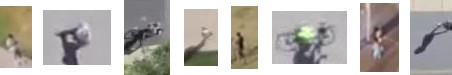
\includegraphics[width=.99\textwidth]{cropped_objects.jpg}
    \caption[Výřezy detekovaných osob neuronovou sítí]{Výřezy detekovaných osob neuronovou sítí.}
    \label{fig_obj_examples}
\end{figure}

Díky výše zmíněným skutečnostem je zvolen jednodušší a přímočařejší přístup, a sice extrakce příznaků pomocí \textbf{barevných histogramů}. Každé detekované osobě ve snímku bude spočítán barevný histogram~--~jak jsou jednotlivé barevné kanály v~daném segmentu rozloženy. Barevný histogram bude sloužit jako příznakový vektor (\textit{feature vector}). Jedná se o~seznam hodnot, který popisuje konkrétní obrázek a může být porovnáván s~jinými příznakovými vektory. Detekované osoby, kterým bude spočítán barevný histogram, budou označeny jako viděné a jejich příznakové vektory budou uloženy. V~dalším snímku budou opět vypočítány příznakové vektory pro každého detekovaného chodce. Následně budou porovnávány s~příznakovými vektory již viděných chodců. Pokud bude nalezena dostatečná shoda, chodec bude považován za reidentifikovaného, jeho příznakový vektor bude nahrazen aktuálnějším a jeho souřadnice v~aktuálním snímku budou uloženy.

\begin{figure}[H]
    \centering
    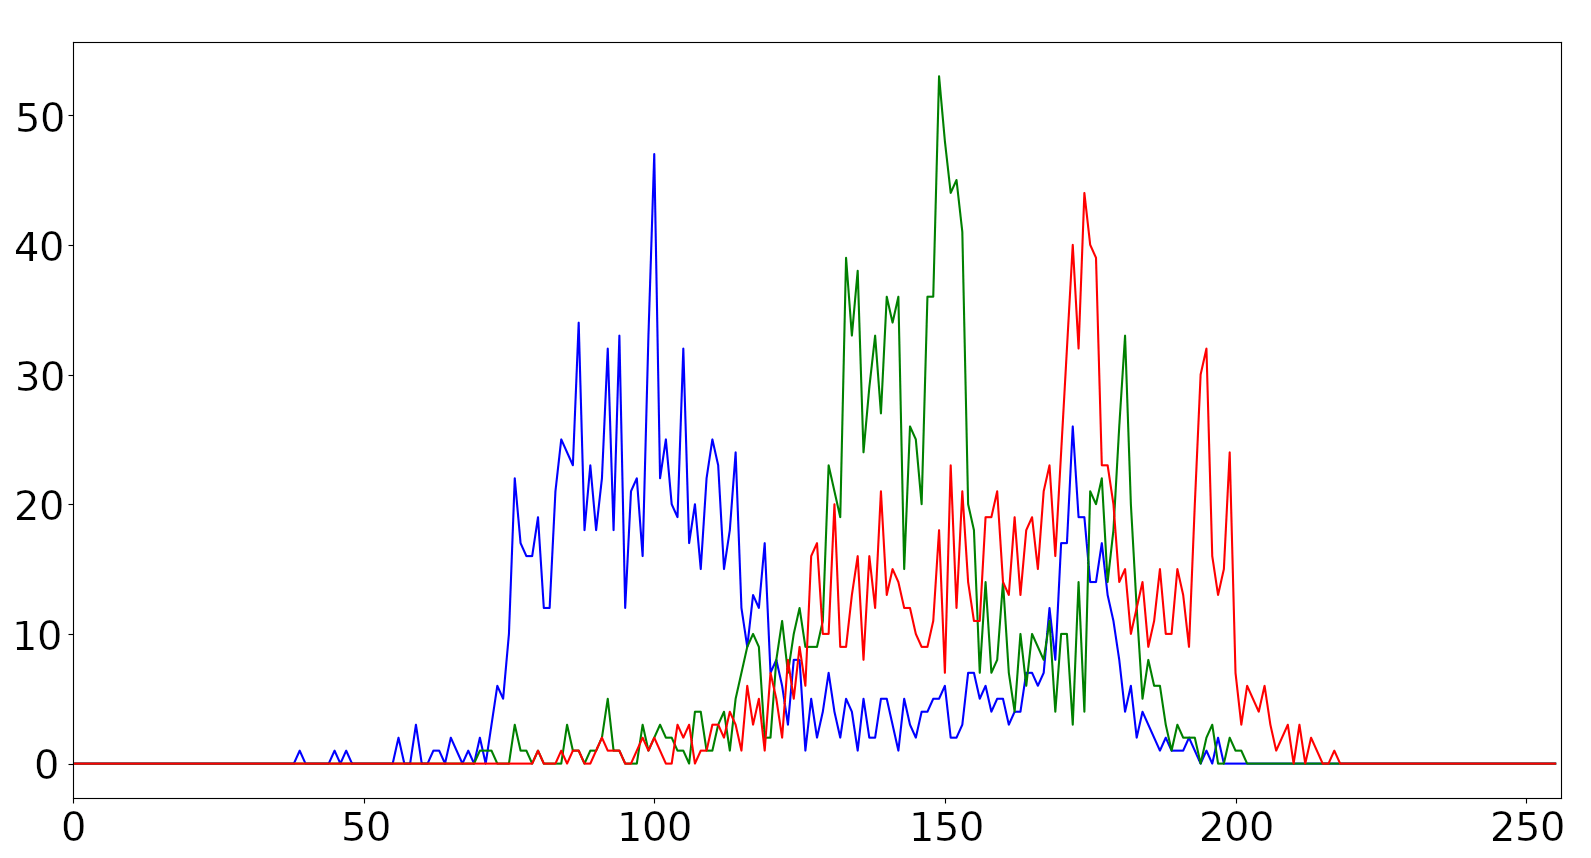
\includegraphics[width=.75\textwidth]{rgb_histogram.png}
    \caption[Příklad RGB histogramu]{RGB histogram jednotlivých barevných složek pro první osobu zleva z~obrázku~\ref{fig_obj_examples}. Na ose $x$ je vyznačeno 256~možných hodnot jednotlivých barevných složek. Na ose $y$ počet pixelů s~touto barevnou hodnotou.}
    \label{fig_histogram}
\end{figure}

Výsledná aplikace People Detector pak bude fungovat následovně. Uživatel přes grafické uživatelské rozhraní specifikuje vstup a spustí detekci. Aplikační okno dávkuje vstupní soubor po jednotlivých snímcích a postupně je předává detektoru. Ten v~každém snímku detekuje osoby, vyřízne je a předá matcheru. Matcher předává výřezy dále describeru, který mu vrací příznakové vektory. Matcher příznakové vektory ukládá a porovnává. Po zpracování všech výřezů vizualizuje trajektorie chodců a výslednou mapu předá detektoru. Uživatel poté může pokračovat v~práci s~aplikací. Například si výstup uložit, zadat nový soubor či spustit detekci znovu. Návrhový diagram celé aplikace je na obrázku~\ref{fig_app_schema}.

\begin{figure}[H]
    \centering
    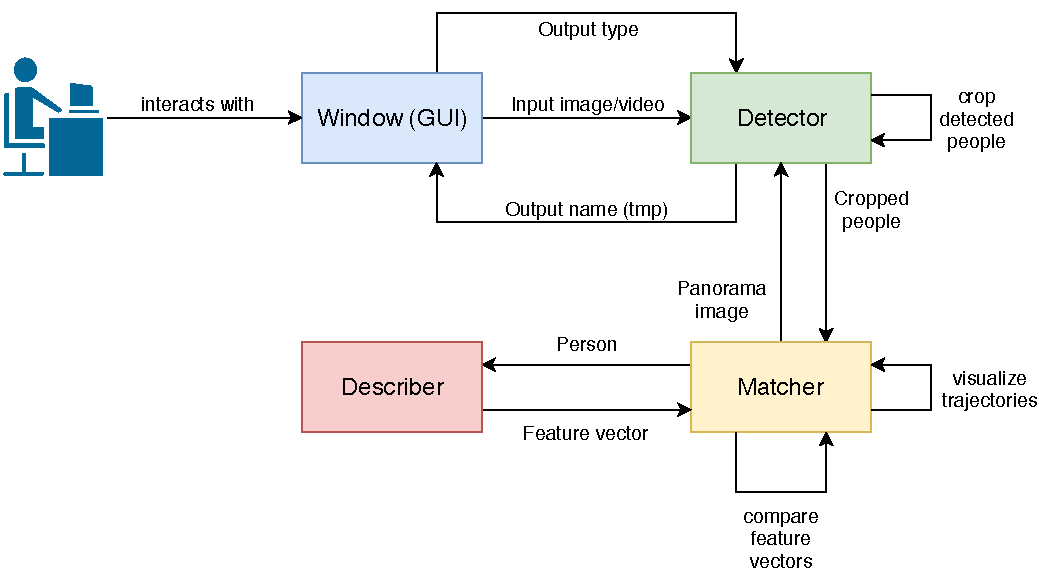
\includegraphics[width=.99\textwidth]{app_schema.pdf}
    \caption[Návrhový diagram aplikace People Detector]{Návrhový diagram aplikace People Detector.}
    \label{fig_app_schema}
\end{figure}

%===============================================================================

\section{Implementace algoritmu}
\label{sec_identification}

Po spuštění aplikace je vytvořena instance detektoru, která načte natrénovaný model sítě RetinaNet ve formátu h5. Výchozí cesta je nastavena k~natrénovanému modelu po 40.~epoše z~třetího trénování, které bylo popsáno v~sekci~\ref{sec_training_process}. Použitý model ale není problém změnit. Lze tak libovolně využít jiný natrénovaný model, stačí specifikovat cestu v~detektoru.

Uživatel interaguje s~aplikací přes její grafické uživatelské rozhraní. Zadá cestu ke vstupnímu souboru (obrázek nebo video ve formátu jpg, jpeg, png, bmp, mp4, avi, wmv, mov nebo mkv) a vybere typ výstupu. Má na výběr ze dvou možností: Za~1. vizualizovat pouze ohraničující obdélníky kolem lidí a zobrazit pravděpodobnost, jak moc si je aplikace jejich detekcí jistá nebo za~2. vizualizovat trajektorie, kudy se osoba napříč videem pohybovala. 2. možnost pochopitelně nemá smysl v~kombinaci s~obrázkem na vstupu.

Pokud uživatel zadá jako vstup video, je třeba, aby bylo detektoru předáváno po snímcích. To je realizováno následujícím algoritmem.

\begin{minipage}{\linewidth}
    \bigskip
    \lstset{caption={Funkce v~pseudokódu Pythonu pro zpracování vstupu v~detektoru.}}
    \begin{lstlisting}
def process_video(window, input_file, output_type):
    for frame in input_file:
        window.actualize_input_label(frame)
        objects_detected = detect_objects(frame)
        image_with_boxes = draw_bounding_boxes(frame, objects_detected)
        if output_type == BORDERS:
            out_file.write(image_with_boxes)
        elif output_type == PANORAMA:
            objects_cropped = crop_objects(frame, objects_detected)
            matcher.process_objects(frame, objects_cropped)
        window.actualize_output_label(image_with_boxes)
        window.progress_bar += step
    if output_type == PANORAMA:
        panorama_image = matcher.get_panorama()
        window.actualize_output_label(panorama_image)
    \end{lstlisting}
\end{minipage}

Po zadání vstupů uživatel spustí detekci. Okno aplikace dávkuje vstupní soubor po snímcích a ty postupně předává detektoru. Detektor pomocí natrénovaného modelu neuronové sítě detekuje ve vstupních datech osoby. Pokud je jako výstup požadováno pouze vyznačení ohraničujících obdélníků, je tak učiněno a výstupní soubor je uložen do dočasného adresáře. Cesta k~němu je předána oknu aplikace v~případě, že by si uživatel přál výstup uložit. Pokud je jako výstup požadovaný panoramatický snímek, lidé jsou z~obrazu vyříznuti a jsou předáni matcheru.

Matcher využije describer, aby pomocí barevných histogramů získal vektor příznaků jednotlivých osob. Ty poté porovnává a jejich výskyty zaznamenává do výsledného panoramatického snímku. Ten následně předá detektoru, který výstupní soubor uloží do dočasného adresáře a cestu k~němu předá oknu, odkud si uživatel může soubor uložit.

Není implementován žádný \textit{image stitching} algoritmus pro spojování snímků napříč videem. Trajektorie pohybu lidí jsou vykreslovány do prvního snímku videa. Z~toho plyne zásadní omezení, a sice že pořízené video musí být ze statického bodu~--~dron se v~průběhu pořizování záznamu nesmí hýbat. Každému rozpoznanému chodci jsou propojena všechna místa, kde byl v~průběhu videa identifikován. Kolem chodce je vyznačen ohraničující obdélník (\textit{bounding box}) a z~jeho středu vede linie, kudy se bude dál ve videu pohybovat.

%-------------------------------------------------------------------------------

\section{Extrakce a porovnávání příznakových vektorů}

Skutečně použitý histogram se od toho na obrázku~\ref{fig_histogram} liší. Byl použit třídimenzionální histogram a jednotlivé barevné kanály byly rozděleny do 8~binů. Kategorizace obrazových bodů probíhá následujícím způsobem: Kolik pixelů má hodnotu červené složky z~daného intervalu, zelené z~jiného a modré zase z~jiného. Například červené z~$\big \langle 0, 31 \big \rangle$, zároveň zelené z~$\big \langle 32, 63 \big \rangle$ a modré z~$\big \langle 64, 95 \big \rangle$. Reálný počet binů je tak $8^3 = 512$.

Histogram je následně normalizován, aby velikost rozlišení vstupního snímku nezkreslovala výsledky. Každá hodnota v~histogramu je vydělena maximální možnou hodnotou, tím jsou všechny hodnoty přeškálovány do intervalu $\big \langle 0, 1 \big \rangle$. Pro extrakci histogramů a jejich následnou normalizaci byla použita knihovna OpenCV.

Spočítání podobnosti výřezů obrázků lze realizovat porovnáním jejich příznakových vektorů. Cílem je spočítat jejich vzájemnou vzdálenost. K~tomu lze použít různé distanční metriky, například euklidovskou vzdálenost,

\begin{equation}
    d(u,v) = \sqrt{\sum_{i=1}^{n} (u_i - v_i)^2}
\end{equation}

manhattanskou vzdálenost,

\begin{equation}
    d(u,v) = \sum_{i=1}^{n} \left | u_i - v_i \right |
\end{equation}

nebo korelační vzdálenost,
\begin{equation}
    d(u,v) = \frac{\sum_{i=1}^{n} (u_i - \hat u) (v_i - \hat v)}{\sqrt{ \sum_{i=1}^{n} (u_i - \hat u) \sum_{i=1}^{n} (v_i - \hat v)}}
\end{equation}

kde $u$, $v$ jsou příznakové vektory a $\hat u$, $\hat v$ jsou průměrné hodnoty.

Experimentálně bylo zjištěno, že pro tento typ dat bude nejvhodnější korelační vzdálenost, kde byly rozdíly ve vzdálenostech mezi stejnými objekty napříč snímky vůči jiným objektům nejvýraznější.

%-------------------------------------------------------------------------------

\section{Experimenty s~dílčími částmi algoritmu}

Pro dokončení algoritmu bylo nutné provést několik experimentů, a tím zjistit, zda porovnání pouze příznakových vektorů je dostačující. Hned první experiment (obrázek~\ref{fig_panorama-v1}) ukázal, že tento přístup není ideální. Pokud je ve snímku zachycen větší počet lidí, je pravděpodobné, že si jejich příznakové vektory mohou být velmi podobné, a díky tomu jako nejpodobnější může být vyhodnocen úplně jiný.

\begin{figure}[H]
    \centering
    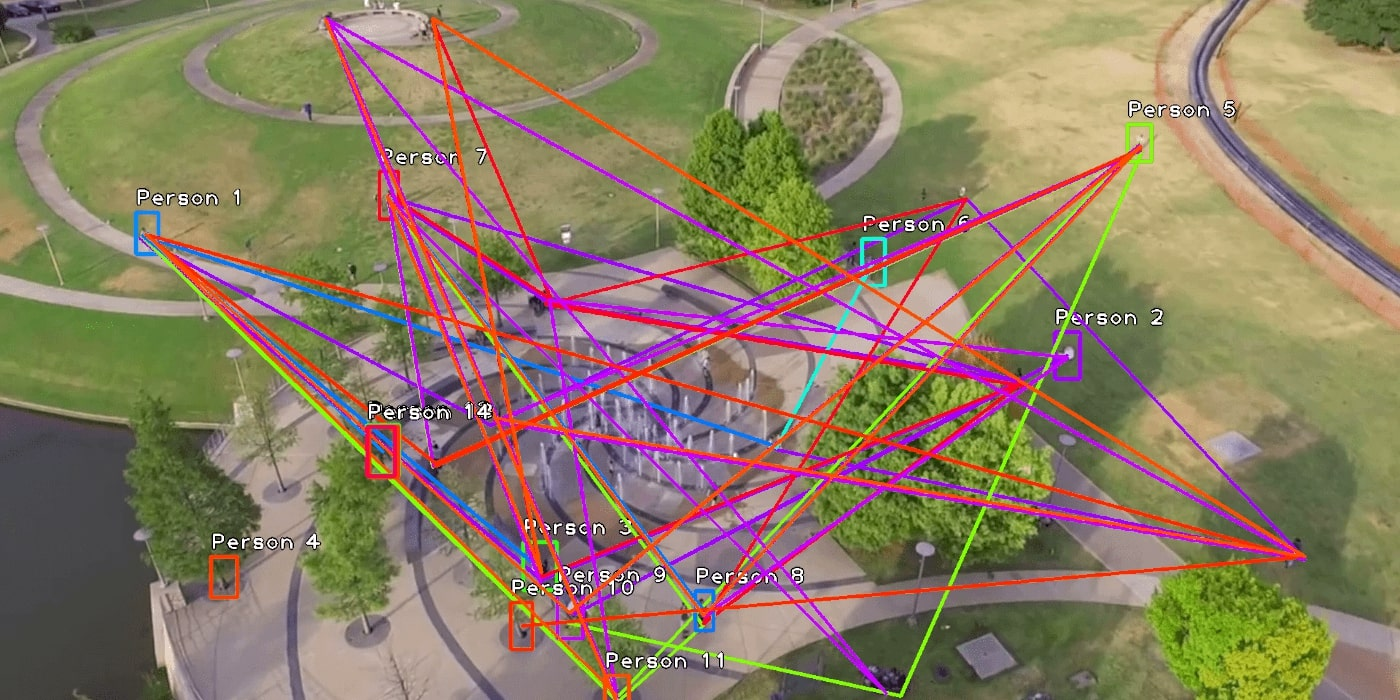
\includegraphics[width=.95\textwidth]{panorama-v1.jpg}
    \caption[První verze algoritmu identifikace chodců]{Vizualizace trajektorií chodců první verzí algoritmu. Chodci jsou porovnáváni pouze na základě příznakových vektorů.}
    \label{fig_panorama-v1}
\end{figure}

Je nemožné, aby se člověk v~rámci jednoho snímku videa přesunul o~výraznou vzdálenost. Vzhledem k~tomu byl algoritmus upraven, aby příznakový vektor osoby byl porovnáván pouze s~příznakovými vektory osob v~její blízkosti. To zajistilo, že detekce nejsou spojovány křížem krážem napříč snímkem. Z~tohoto přístupu vyplývá problém v~následujícím případě: Člověk projde pod nějakou překážkou, a tím se kameře schová. Jeho další detekce, ačkoliv o~spoustu snímků později, může tak být velmi vzdálená od té předchozí. Stejný případ může nastat, pokud člověk záběr opustí a poté se do něho vrátí v~jiném místě.

\begin{figure}[H]
    \centering
    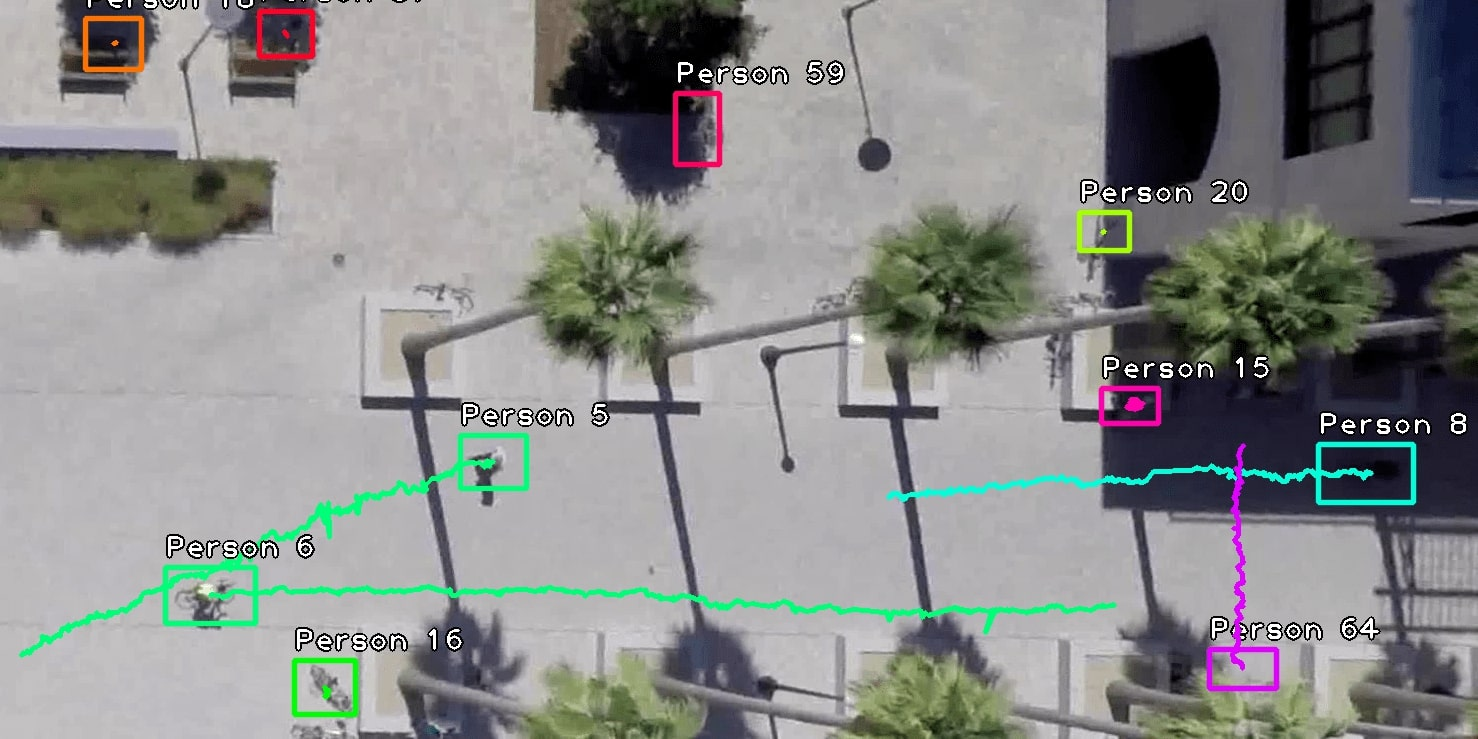
\includegraphics[width=.95\textwidth]{panorama-v2.jpg}
    \caption[Druhá verze algoritmu identifikace chodců]{Vizualizace trajektorií chodců druhou verzí algoritmu. Při porovnávání příznakových vektorů chodců je brána v~potaz i jejich reálná vzdálenost ve snímku.}
    \label{fig_panorama-v2}
\end{figure}

Výsledek nyní vypadá podstatně lépe. Avšak ve snímku jsou vyznačeny statické objekty, které jistě nejsou lidé. To je dáno chybou neuronové sítě, která v~některém snímku vrátila jako osobu objekt, který osoba není. Druhý problém je vidět na osobě~64. Tento člověk se ve videu objevil až později, nebyl na prvním snímku. Proto je zakreslen ohraničující obdélník kolem prázdného místa.

Dá se předpokládat, že ve většině záznamů se lidé budou pohybovat, zvlášť bude-li videozáznam delší. Pokud se člověk pohybovat nebude, nemá pro něho vykreslení trajektorie pohybu smysl. Algoritmus byl upraven tak, aby pro statické objekty, které se v~rámci celého pořízeného záběru nepohnou, nebylo vykresleno nic. Tato úprava vyřešila problém občasné chybné detekce neuronovou sítí nějakého statického objektu jako člověka.

Druhá úprava se pak postarala o~problém prázdných obdélníků pro osoby, které se v~záběru objevily až později. Při jejich prvním výskytu je obraz s~nimi vyříznut a překopírován do panoramatického snímku.

\begin{figure}[H]
    \centering
    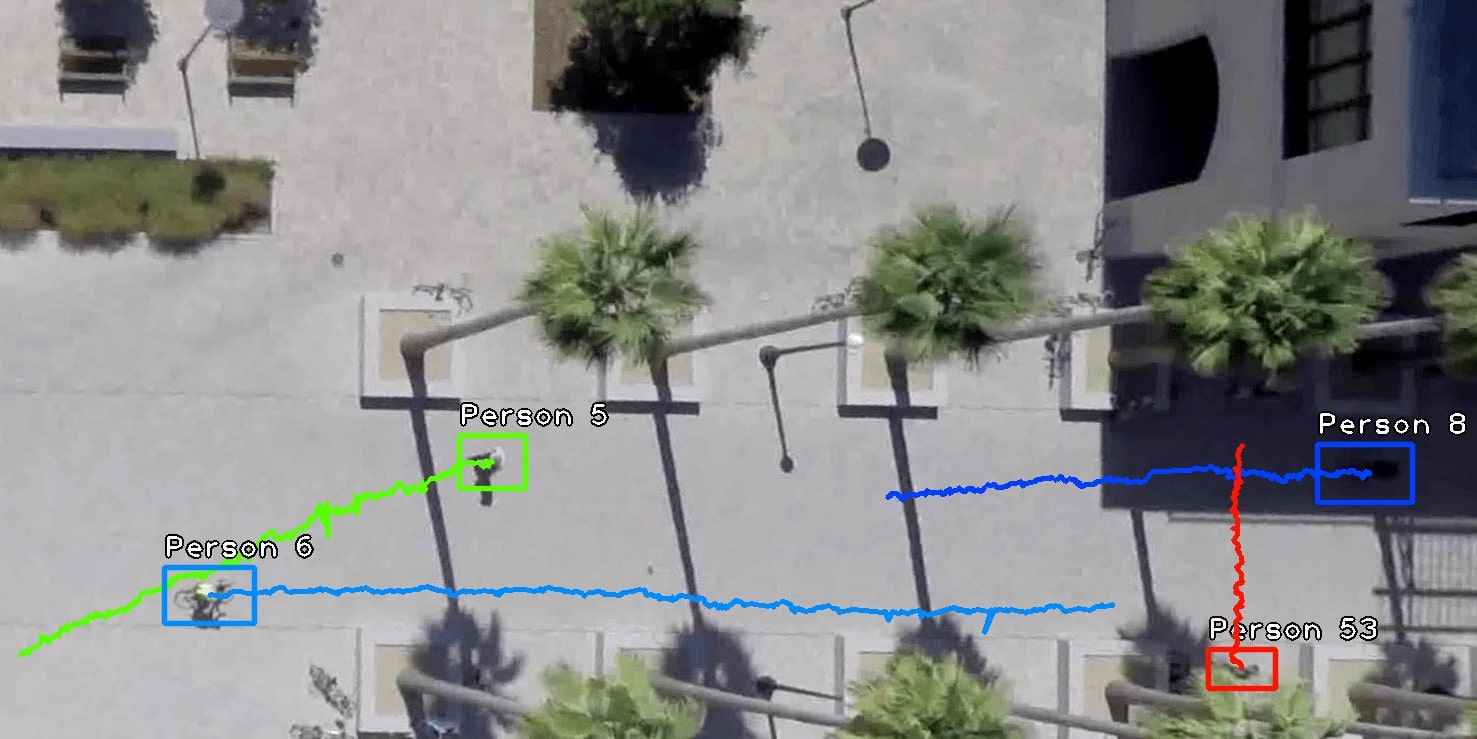
\includegraphics[width=.95\textwidth]{panorama-v3.jpg}
    \caption[Třetí verze algoritmu identifikace chodců]{Vizualizace trajektorií chodců třetí verzí algoritmu. Nyní jsou ve snímku vyznačeni pouze lidé a trajektorie, kterými bude směrován jejich pohyb.}
    \label{fig_panorama-v3}
\end{figure}

Výsledné algoritmy pro zpracování objektů a vykreslení trajektorií jsou zachyceny na následujících výpisech.

\begin{minipage}{\linewidth}
    \bigskip
    \lstset{caption={Výsledná funkce v~pseudokódu Pythonu pro vizualizaci trajektorií.}}
    \begin{lstlisting}
def get_panorama_image(image, known_objects):
    for obj in known_objects:
        if is_static_object(obj):
            continue
        if not detected_in_first_frame(obj):
            insert_cutout_into_image(image, obj.cutout)
        draw_bounding_box(image, obj)
        draw_caption(image, obj)
        previous_point = obj.points.pop(0)
        for point in obj.points:
            draw_line(image, prev_point, point)
            previous_point = point
    return image
    \end{lstlisting}
\end{minipage}

\begin{minipage}{\linewidth}
    \bigskip
    \lstset{caption={Výsledná funkce v~pseudokódu Pythonu pro zpracování objektů detekovaných neuronovou sítí.}}
    \begin{lstlisting}
def process_objects(known_objects, frame, objects):
    for obj in objects:
        if frame == 0:
            obj.compute_histogram()
            obj.detected_in_first_frame = True
            known_objects.append(obj)
        else:
            obj.compute_histogram()
            most_similar_obj = None
            shortest_hist_distance = MAX_INT
            for known_obj in known_objects:
                euclidean_distance = compute_euclidean_distance(obj, known_obj)
                if euclidean_distance < EUCLIDEAN_DISTANCE_TRESHOLD:
                    hist_distance = compute_correlation_distance(obj, known_obj)
                    if hist_distance < shortest_hist_distance:
                        shortest_hist_distance = hist_distance
                        most_similar_obj = known_obj
            if shortest_hist_distance < HIST_SIMILARITY_TRESHOLD:
                most_similar_obj.compute_hist(obj)
                most_similar_obj.add_point(obj)
            else:
                known_objects.append(obj)
    \end{lstlisting}
\end{minipage}

%===============================================================================

\section{Implementace demonstrační aplikace}
\label{sec_implementation}

Pro kompletní otestování funkcionality a provedení experimentů bylo nutné naimplementovat demonstrační aplikaci. Vzhledem k~požadavku na multiplatformnost aplikace byla  brána v~potaz složitost přenosu aplikace na různé operační systémy a s~tím spojené komplikace, se kterými by se uživatel musel vypořádávat při instalaci potřebných závislostí.

Samotná aplikace je naprogramovaná v~jazyce Python v~aktuální verzi~3.7.3. Její vývoj probíhal ve vývojovém prostředí (IDE) PyCharm od společnosti JetBrains. JetBrains poskytují licence ke svému software ve verzi Ultimate pro studenty a akademické účely zdarma.

Grafické uživatelské rozhraní bylo realizováno pomocí knihovny PyQt\footnote{\url{https://www.riverbankcomputing.com/software/pyqt}} ve verzi~4.8.7. PyQt je odnož frameworku Qt pro implementaci uživatelských rozhraní v~Pythonu. Qt je široce používaný multiplatformní framework, ve kterém lze vyvíjet aplikace v~odlišných programovacích jazycích pro různé platformy.

Pro otevírání, ukládání a manipulaci s~obrázky byla využita knihovna PIL (Python Imaging Library). Konkrétně její fork Pillow\footnote{\url{https://pillow.readthedocs.io/en/stable/}} verze~6.0.0, který od Pythonu verze~3 nahradil původní implementaci, jelikož její vývoj byl ukončen.

Použitá implementace detekční sítě RetinaNet, která byla blíže popsána v~sekci~\ref{sec_retinanet_implementation}, vyžaduje knihovnu Keras\footnote{\url{https://keras.io/}} verze~2.2.4 nebo novější. Ta je dostupná buď samostatně nebo přímo jako součást Tensorflow\footnote{\url{https://www.tensorflow.org/}} od verze~1.13.

Pro načítání, zpracování obrazových dat, manipulaci s~video soubory, počítání a normalizací barevných histogramů a vizualizaci ohraničujících boxů či trajektorií byla použita knihovna OpenCV\footnote{\url{https://opencv.org/}} verze~4.1.0.

Počítání distančních metrik mezi vektory příznaků bylo realizováno pomocí knihovny SciPy\footnote{\url{https://www.scipy.org/}} ve verzi~1.2.1.

Výše zmíněné knihovny pracují s~reprezentací obrazových dat jako s~multidimenzionálním polem. Konkrétně s~polem NumPy array a operacemi implementovanými nad ním v~knihovně NumPy\footnote{\url{https://www.numpy.org/}}. Použita byla aktuální verze~1.16.3.

Veškeré použité nástroje jsou platformně nezávislé. Aplikaci by tak neměl být problém spustit na většině operačních systémů. Potřebné Python knihovny je možné doinstalovat pomocí správce balíků (\textit{package manager}) Pip z~oficiálního repozitáře PyPI (Python Package Index). Výjimku tvoří pouze knihovna PyQt, která zastává pouze funkci wrapperu nad C++ implementací Qt. Python knihovna tak poskytuje pouze pohodlné rozhraní pro práci s~ní. Z~toho důvodu je třeba ji instalovat přes správce balíků operačního systému. Například přes DNF v~případě linuxových distribucí založených na RPM nebo přes APT v~případě distribucí založených na Debian. Pro účely této práce byla aplikace otestována na operačním systému Fedora~29, Ubuntu~18.04 a Windows~10 (Verze~1809, OS~Build~17763.437).

%-------------------------------------------------------------------------------

\subsection*{Grafické uživatelské rozhraní}

Grafické uživatelské rozhraní poskytuje tři tlačítka (\textit{push button}) pro základní ovládání aplikace. Otevření vstupního souboru, spuštění procesu detekce a uložení výstupu. Všechny tyto akce jsou přístupné i z~hlavního menu (\textit{menu bar}) nebo přes klávesové zkratky. Posledním ovládacím prvkem je přepínač (\textit{radio button}) mezi typy výstupů.

\begin{figure}[H]
    \centering
    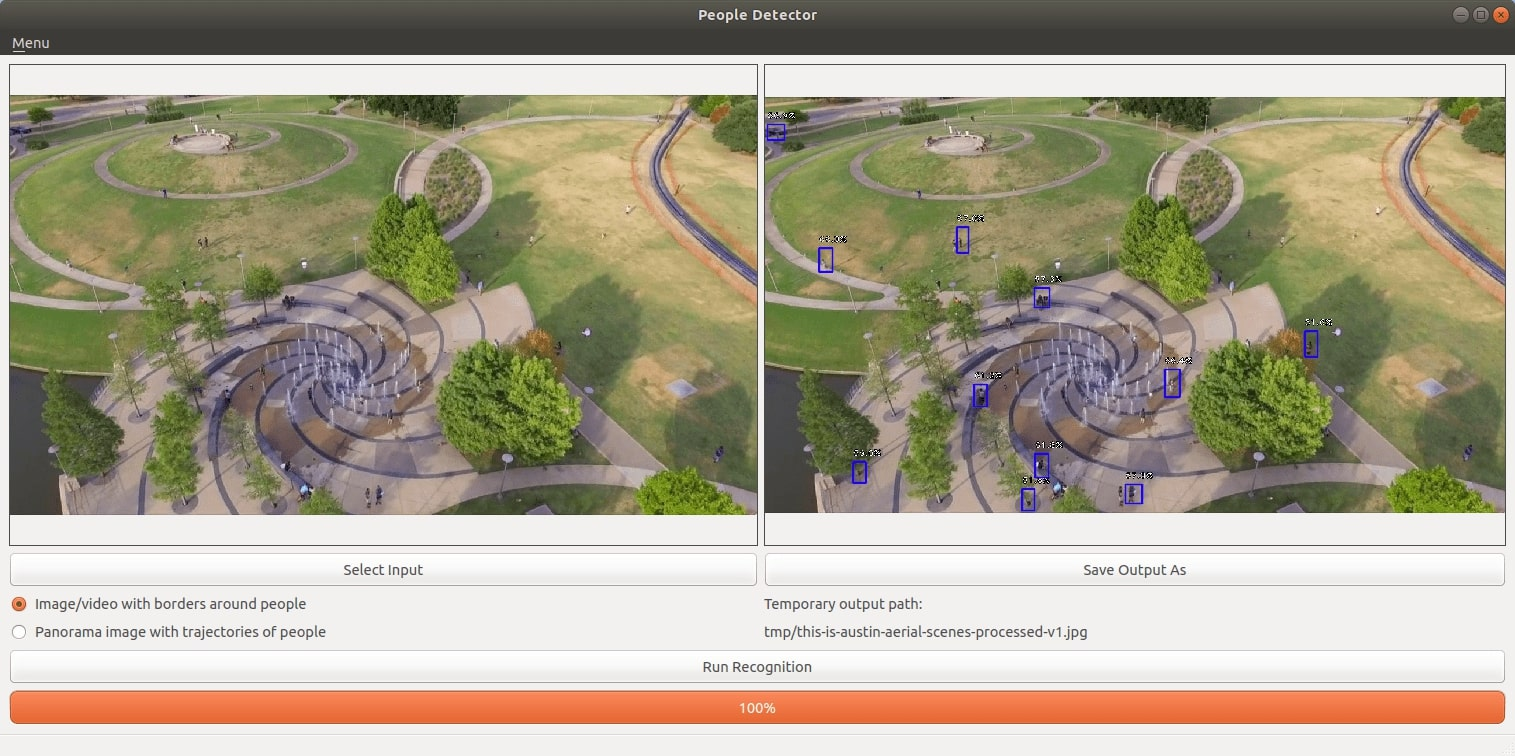
\includegraphics[width=.99\textwidth]{gui-1.jpg}
    \caption[Ukázka grafického rozhraní aplikace People Detector]{Ukázka využití aplikace přes jeho grafické uživatelské rozhraní. Jako vstup je zvolen snímek a typ výstupu snímek s~ohraničujícími obdélníky kolem lidí. Uživatel si nyní může výstup uložit, zvolit další vstup nebo jenom změnit typ výstupu a spustit rozpoznávání znovu.}
    \label{fig_gui-1}
\end{figure}

Aplikace také obsahuje štítky (\textit{label}) pro vizualizaci vstupních a výstupních dat. V~případě, že je na vstupu vybráno video, jsou štítky při každém zpracovaném snímku aktualizovány. Uživatel tak může v~průběhu procesu zpracování pozorovat, jak je aplikace s~detekcí úspěšná.

\begin{figure}[H]
    \centering
    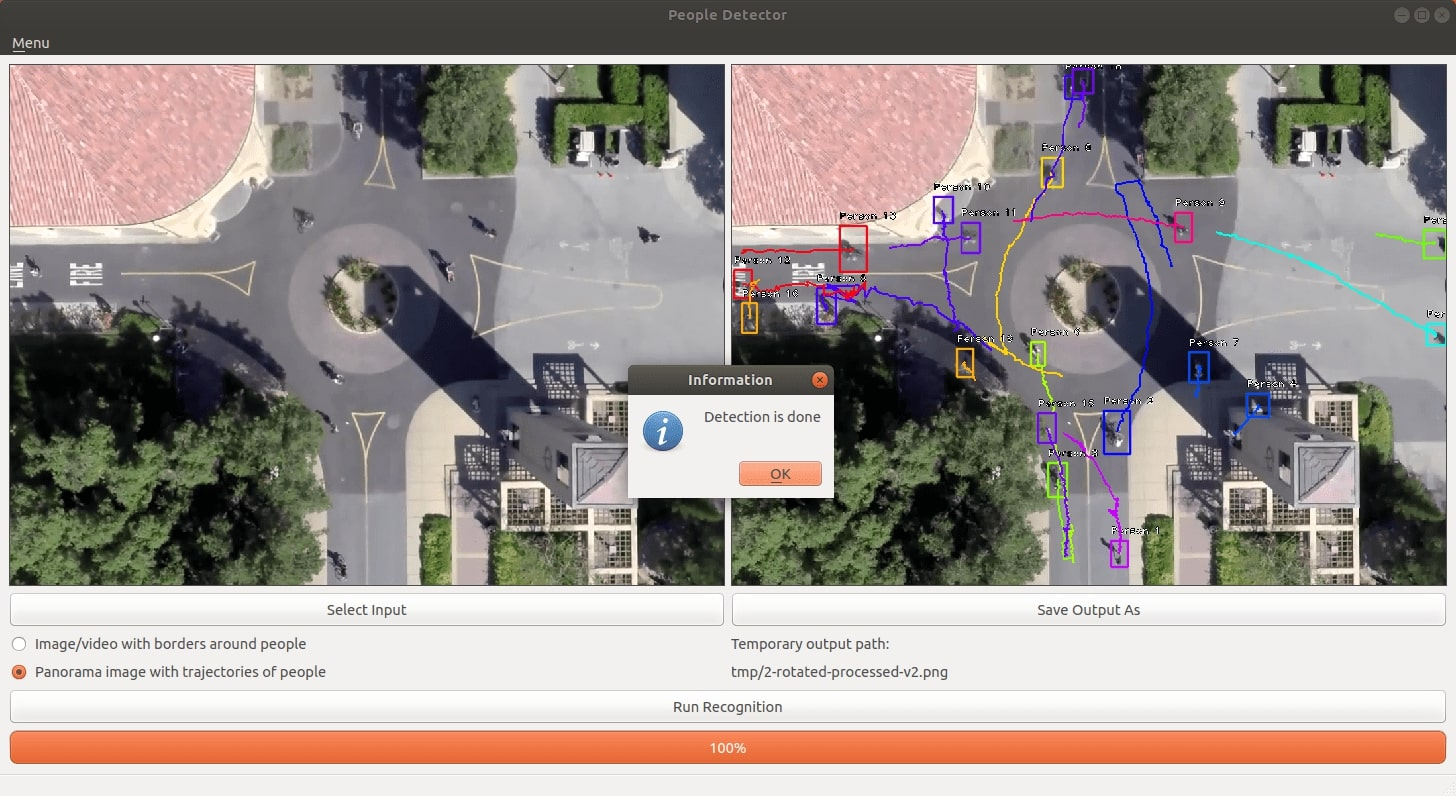
\includegraphics[width=.99\textwidth]{gui-2.jpg}
    \caption[Další ukázka grafického rozhraní aplikace People Detector]{Další ukázka použití aplikace. Tentokrát je jako vstup zvoleno video a výstup panoramatická mapa.}
    \label{fig_gui-2}
\end{figure}

Posledním prvkem grafického rozhraní je ukazatel průběhu zpracování vstupu (\textit{progress bar}). Předem je spočítána velikost kroku, o~který se ukazatel bude posunovat. Ta je odvozena od počtu snímků ve videu. Po každém zpracovaném snímku se pak ukazatel o~danou velikost kroku posune. Při zpracování fotky nabývá ukazatel pouze hodnot~0\,\% a~100\,\%.

%===============================================================================
